\documentclass[11pt]{article}
\usepackage[a4paper,margin=1in]{geometry}
\usepackage[T1]{fontenc}
\usepackage{lmodern}
\usepackage{microtype}
\usepackage{amsmath}
\usepackage{booktabs}
\usepackage{graphicx}
\usepackage{fancyhdr}
\usepackage[hidelinks]{hyperref}

\pagestyle{fancy}
\fancyhf{}
\renewcommand{\headrulewidth}{0pt}
\fancyfoot[L]{ET23BTIT133}
\fancyfoot[R]{\thepage}

\begin{document}
\begin{center}
{\LARGE\bfseries Supervised Machine Learning Approach for\\
WSD in Spoken News\par}
\vspace{0.8em}
{\Large Evaluation Report\par}
\vspace{0.8em}
{\large Sree Saicharan Vadapalli\\ ET23BTIT133\par}
\end{center}
\vspace{1em}

\section{Setup}

Everything here comes from one run of \texttt{src/pipeline.py}: 8 target words,
1,092 SemCor occurrences, a linear SVM and multinomial Naive Bayes, and window
sizes $W = \pm 2$ and $W = \pm 5$. Scores are from stratified 5-fold
cross-validation, so each occurrence is predicted once by a model that did not
train on it. The Architecture and Methodology document covers the features and
the protocol in detail.

\section{Results}

Table~\ref{tab:results} has the per-word scores. ``Majority'' is the share of
the most common sense, i.e.\ the accuracy you would get by always guessing it.

\begin{table}[h]
\centering
\small
\begin{tabular}{lrrr cccc cccc}
\toprule
& & & & \multicolumn{4}{c}{SVM} & \multicolumn{4}{c}{Naive Bayes} \\
\cmidrule(lr){5-8} \cmidrule(lr){9-12}
& & & & \multicolumn{2}{c}{Accuracy} & \multicolumn{2}{c}{Macro F1}
& \multicolumn{2}{c}{Accuracy} & \multicolumn{2}{c}{Macro F1} \\
Word & $n$ & Senses & Majority & $\pm2$ & $\pm5$ & $\pm2$ & $\pm5$
& $\pm2$ & $\pm5$ & $\pm2$ & $\pm5$ \\
\midrule
bank & 34 & 2 & 0.59 & 0.68 & 0.79 & 0.68 & 0.78 & 0.62 & 0.76 & 0.61 & 0.76 \\
case & 133 & 5 & 0.48 & 0.54 & 0.55 & 0.36 & 0.34 & 0.52 & 0.56 & 0.24 & 0.28 \\
interest & 140 & 7 & 0.41 & 0.61 & 0.59 & 0.47 & 0.37 & 0.54 & 0.50 & 0.23
& 0.27 \\
plant & 107 & 3 & 0.59 & 0.69 & 0.70 & 0.63 & 0.54 & 0.69 & 0.65 & 0.62 & 0.49
\\
power & 99 & 6 & 0.57 & 0.63 & 0.63 & 0.49 & 0.41 & 0.59 & 0.61 & 0.20 & 0.26 \\
rate & 116 & 3 & 0.59 & 0.88 & 0.85 & 0.82 & 0.74 & 0.84 & 0.83 & 0.70 & 0.57 \\
run & 185 & 12 & 0.36 & 0.49 & 0.48 & 0.31 & 0.29 & 0.46 & 0.46 & 0.16 & 0.19 \\
state & 278 & 6 & 0.39 & 0.72 & 0.71 & 0.57 & 0.52 & 0.68 & 0.67 & 0.45
& 0.44 \\
\midrule
Overall & 1092 & & & 0.65 & 0.64 & 0.54 & 0.50 & 0.61 & 0.61 & 0.40 & 0.41 \\
\bottomrule
\end{tabular}
\caption{Per-word results. The overall row is accuracy pooled over all
occurrences and macro F1 averaged over words.}
\label{tab:results}
\end{table}

Both models beat the majority-sense guess on every word, and the SVM is the
better of the two overall. The gap between accuracy and macro F1 is large for
most words, which says the models get the common senses right and struggle
with the rare ones.

\section{Window size impact}

\begin{figure}[h]
\centering
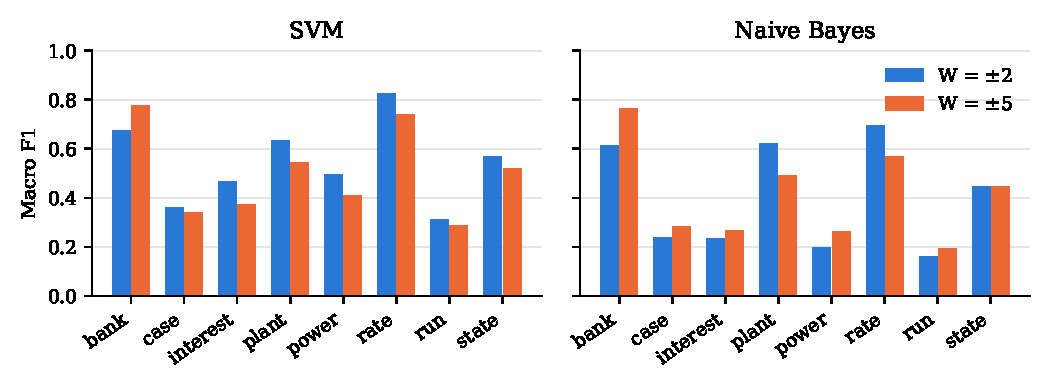
\includegraphics[width=\linewidth]{figures/window_f1.pdf}
\caption{Macro F1 per word at both window sizes.}
\label{fig:window}
\end{figure}

A wider window does not help in general. For the SVM, overall accuracy barely
moves (0.65 to 0.64) and macro F1 drops from 0.54 to 0.50. Most of that drop
comes from \emph{interest}, \emph{plant}, \emph{power} and \emph{rate}, where
macro F1 falls by 0.08 to 0.09 each. Naive Bayes is mixed: it gains a little on
\emph{bank}, \emph{case}, \emph{interest}, \emph{power} and \emph{run} and loses
on \emph{plant} and \emph{rate}, ending about flat overall.

The reason is that the useful cues for most of these words are local. Phrases
like ``interest rate'', ``rate of'' or ``power plant'' sit right next to the
target and are already inside $\pm 2$. Going to $\pm 5$ gives two to three
times as many features, most of them words that show up once or twice, and with
100 to 300 examples per word that is mostly noise for the SVM to fit.

\emph{bank} is the exception and the clearest win for $\pm 5$ (SVM accuracy
0.68 to 0.79). Its two senses, the financial institution and the river bank,
are about topic rather than local syntax. In ``the board of directors of the
\textbf{bank} with the approval of the Farm Credit Administration'', the $\pm 2$
window sees only ``of the'' and ``with the''; at $\pm 5$ it reaches
``directors'' and ``approval'' and gets it right.

\section{SVM vs Naive Bayes}

At $W = \pm 2$ the SVM has higher accuracy on every word except \emph{plant},
where they tie. At $\pm 5$ Naive Bayes edges ahead on \emph{case} (0.56 vs 0.55)
but is behind everywhere else. The bigger difference is in macro F1,
0.54 vs 0.40 at $\pm 2$. On words with many senses, Naive Bayes falls back on
the prior and predicts the majority sense most of the time: its macro F1 is
0.23 on \emph{interest}, 0.20 on \emph{power} and 0.16 on \emph{run}. The
features are heavily correlated (the same context shows up as POS tags and as
words), and the independence assumption counts that evidence several times,
which likely pushes Naive Bayes towards overconfident, majority-leaning
predictions.
The SVM learns weights jointly and handles the redundancy better.

\section{Failure analysis}

Table~\ref{tab:plant} shows where the SVM goes wrong on \emph{plant} at
$W = \pm 2$.

\begin{table}[h]
\centering
\small
\begin{tabular}{lccc}
\toprule
& \multicolumn{3}{c}{Predicted} \\
\cmidrule(lr){2-4}
Gold & plant.n.01 (factory) & plant.n.02 (organism) & plant.v.01 (to plant) \\
\midrule
plant.n.01 (factory) & 50 & 13 & 0 \\
plant.n.02 (organism) & 15 & 21 & 0 \\
plant.v.01 (to plant) & 5 & 0 & 3 \\
\bottomrule
\end{tabular}
\caption{SVM confusion matrix for \emph{plant}, $W = \pm 2$.}
\label{tab:plant}
\end{table}

\paragraph{Too little context in the window.} Many factory/organism confusions
are occurrences like ``cut it off from the mother \textbf{plant}'' or ``into
each hole with the \textbf{plant}'', where the $\pm 2$ window is mostly
determiners and punctuation. With no content words to go on, the model falls
back to the majority sense.

\paragraph{Rare senses get outvoted.} Five of the eight verb uses of
\emph{plant} are tagged as the factory sense even though the POS feature marks
them as verbs. With about six verb examples per training fold, the model does
not put enough weight on the target POS to override everything else. The same
thing happens with \emph{interest.v.01}, where 4 of its 5 occurrences get a
noun sense.

\paragraph{Fine-grained WordNet senses.} Some errors are distinctions that are
hard even for people. ``Insurance \textbf{rates}'' and ``hospital
\textbf{rates}'' are gold \emph{rate.n.02} (an amount charged) and get
predicted as \emph{rate.n.01} (a magnitude relative to something). For
\emph{interest}, 28 of the 55 errors are other senses predicted as
\emph{interest.n.01} (curiosity), for example \emph{interest.n.03} (the quality
of being interesting) in ``features of \textbf{interest}''. This includes the
financial sense \emph{interest.n.04}, which matters most for news and is right
only 2 times out of 14.

\section{Limitations}

\begin{itemize}
\item SemCor is written text. Real transcripts have no punctuation or casing and
contain recognition errors, which will hurt the POS tagger and through it the
POS features. Expect lower numbers on actual spoken news.
\item The data is small. \emph{bank} has only 34 usable occurrences, so a
difference of one prediction moves its accuracy by about 0.03.
\item Both classifiers use default hyperparameters, and results are from a
single cross-validation seed.
\end{itemize}

\section{Conclusion}

A linear SVM over target POS, neighbouring POS and a $\pm 2$ bag-of-words works
best here, with 0.65 accuracy and 0.54 macro F1 overall. Widening the window to
$\pm 5$ only pays off for words whose senses are topical, like \emph{bank}; for
the rest it adds noise. Naive Bayes is close on accuracy but much worse on
rare senses. The main sources of error are short, uninformative windows,
senses with very few examples, and WordNet distinctions that are finer than the
context can resolve.

\end{document}
